\let\negmedspace\undefined
\let\negthickspace\undefined
\documentclass[journal]{IEEEtran}
\usepackage[a5paper, margin=10mm, onecolumn]{geometry}
%\usepackage{lmodern} % Ensure lmodern is loaded for pdflatex
\usepackage{tfrupee} % Include tfrupee package

\setlength{\headheight}{1cm} % Set the height of the header box
\setlength{\headsep}{0mm}     % Set the distance between the header box and the top of the text

\usepackage{gvv-book}
\usepackage{gvv}
\usepackage{cite}
\usepackage{amsmath,amssymb,amsfonts,amsthm}
\usepackage{algorithmic}
\usepackage{graphicx}
\usepackage{textcomp}
\usepackage{xcolor}
\usepackage{txfonts}
\usepackage{listings}
\usepackage{enumitem}
\usepackage{mathtools}
\usepackage{gensymb}
\usepackage{comment}
\usepackage[breaklinks=true]{hyperref}
\usepackage{tkz-euclide} 
\usepackage{listings}
% \usepackage{gvv}                                        
\def\inputGnumericTable{}                                 
\usepackage[latin1]{inputenc}                                
\usepackage{color}                                            
\usepackage{array}                                            
\usepackage{longtable}                                       
\usepackage{calc}                                             
\usepackage{multirow}                                         
\usepackage{hhline}                                           
\usepackage{ifthen}                                           
\usepackage{lscape}
\begin{document}

\bibliographystyle{IEEEtran}
\vspace{3cm}

\title{10.3.3.2}
\author{EE24BTECH11034 - K Teja Vardhan}
% \maketitle
% \newpage
% \bigskip
{\let\newpage\relax\maketitle}

\renewcommand{\thefigure}{\theenumi}
\renewcommand{\thetable}{\theenumi}
\setlength{\intextsep}{10pt} % Space between text and floats

\numberwithin{figure}{enumi}
\renewcommand{\thetable}{\theenumi}

\section{Problem Statement}
The difference of two supplementary angles by 18, find the angles.
\section{equations}
since they are supplementary and their difference is 18 hence the equations are,
\[
\begin{aligned}
    x + y &= 180, \\
    x - y &= 18.
\end{aligned}
\]
Our goal is to solve for \(x\) and \(y\) using multiple methods.

\section{Substitution Method}
\subsection*{Step 1: Solve one equation for one variable}
From the first equation:
\begin{align}
    x + y &= 180, \\
    y &= 180 - x.
\end{align}

\subsection*{Step 2: Substitute into the second equation}
Substitute \(y = 180 - x\) into the second equation:
\begin{align}
    x - (180 - x) &= 18, \\
    x - 180 + x &= 18, \\
    2x - 180 &= 18.
\end{align}

\subsection*{Step 3: Solve for \(x\)}
\begin{align}
    2x &= 198, \\
    x &= 99.
\end{align}

\subsection*{Step 4: Substitute back to find \(y\)}
Substitute \(x = 99\) into \(y = 180 - x\):
\begin{align}
    y &= 180 - 99, \\
    y &= 81.
\end{align}

\subsection*{Final Solution}
\[\boxed{x = 99, \quad y = 81.}\]

\section{Elimination Method}
\subsection*{Step 1: Add the two equations}
Add the two equations to eliminate \(y\):
\begin{align}
    (x + y) + (x - y) &= 180 + 18, \\
    2x &= 198, \\
    x &= 99.
\end{align}

\subsection*{Step 2: Substitute \(x\) into one equation}
Substitute \(x = 99\) into \(x + y = 180\):
\begin{align}
    99 + y &= 180, \\
    y &= 180 - 99, \\
    y &= 81.
\end{align}

\subsection*{Final Solution}
\[\boxed{x = 99, \quad y = 81.}\]

\section{Matrix Method}
\subsection*{Step 1: Represent the system in matrix form}
\begin{align}
    \begin{bmatrix} 1 & 1 \\ 1 & -1 \end{bmatrix}
    \begin{bmatrix} x \\ y \end{bmatrix} &=
    \begin{bmatrix} 180 \\ 18 \end{bmatrix}.
\end{align}
Let \(A = \begin{bmatrix} 1 & 1 \\ 1 & -1 \end{bmatrix}\), \(X = \begin{bmatrix} x \\ y \end{bmatrix}\), and \(B = \begin{bmatrix} 180 \\ 18 \end{bmatrix}\).

\subsection*{Step 2: Compute the determinant of \(A\)}
\begin{align}
    \det(A) &= \begin{vmatrix} 1 & 1 \\ 1 & -1 \end{vmatrix}, \\
    &= (1 \times -1) - (1 \times 1), \\
    &= -1 - 1 = -2.
\end{align}

\subsection*{Step 3: Find \(A^{-1}\)}
\begin{align}
    A^{-1} &= \frac{1}{\det(A)} \begin{bmatrix} -1 & -1 \\ -1 & 1 \end{bmatrix}, \\
    &= \frac{1}{-2} \begin{bmatrix} -1 & -1 \\ -1 & 1 \end{bmatrix}, \\
    &= \begin{bmatrix} \frac{1}{2} & \frac{1}{2} \\
    \frac{1}{2} & -\frac{1}{2} \end{bmatrix}.
\end{align}

\subsection*{Step 4: Multiply \(A^{-1}\) by \(B\)}
\begin{align}
    X &= A^{-1} B, \\
    &= \begin{bmatrix} \frac{1}{2} & \frac{1}{2} \\
    \frac{1}{2} & -\frac{1}{2} \end{bmatrix}
    \begin{bmatrix} 180 \\ 18 \end{bmatrix}, \\
    &= \begin{bmatrix} 99 \\ 81 \end{bmatrix}.
\end{align}

\subsection*{Final Solution}
\[\boxed{x = 99, \quad y = 81.}\]

\section{Cramer's Rule}
\subsection*{Step 1: Compute \(\det(A)\)}
\begin{align}
    \det(A) &= -2.
\end{align}

\subsection*{Step 2: Compute \(\det(A_x)\) and \(\det(A_y)\)}
Replace the first and second columns of \(A\) with \(B\):
\begin{align}
    \det(A_x) &= \begin{vmatrix} 180 & 1 \\ 18 & -1 \end{vmatrix}, \\
    &= (180 \times -1) - (1 \times 18) = -198, \\
    \det(A_y) &= \begin{vmatrix} 1 & 180 \\ 1 & 18 \end{vmatrix}, \\
    &= (1 \times 18) - (180 \times 1) = -162.
\end{align}

\subsection*{Step 3: Solve for \(x\) and \(y\)}
\begin{align}
    x &= \frac{\det(A_x)}{\det(A)} = \frac{-198}{-2} = 99, \\
    y &= \frac{\det(A_y)}{\det(A)} = \frac{-162}{-2} = 81.
\end{align}

\subsection*{Final Solution}
\[\boxed{x = 99, \quad y = 81.}\]

\section{Gaussian Elimination}
\subsection*{Step 1: Augmented Matrix Representation}
\begin{align}
    \begin{bmatrix} 1 & 1 & | & 180 \\
                  1 & -1 & | & 18 \end{bmatrix}
\end{align}

\subsection*{Step 2: Forward Elimination}
Eliminate \(x\) from the second row:
\begin{align}
    R_2 &\to R_2 - R_1, \\
    \begin{bmatrix} 1 & 1 & | & 180 \\
                  0 & -2 & | & -162 \end{bmatrix}.
\end{align}

\subsection*{Step 3: Back Substitution}
Solve for \(y\) from the second row:
\begin{align}
    -2y &= -162, \\
    y &= 81.
\end{align}
Substitute \(y = 81\) into the first row:
\begin{align}
    x + 81 &= 180, \\
    x &= 99.
\end{align}

\subsection*{Final Solution}
\[\boxed{x = 99, \quad y = 81.}\]

\section*{Solving a System of Linear Equations Using Computational Methods}

We are solving the system of equations:
\begin{align}
x + y &= 180, \\
x - y &= 18.
\end{align}

Rewriting the equations:
\begin{align}
x &= 180 - y, \\
y &= 18 + x.
\end{align}

First, we rewrite the question as a system of linear equations.
\begin{align}
    x_1 &\implies x, \\
    x_2 &\implies y
\end{align}

Converting into matrix form, we get:
\begin{align}
    \myvec{1 & 1\\ 1 & -1}\myvec{x_1 \\\ x_2} &= \myvec{180 \\\ 18} \\
    \vec{A}x &= \vec{b}
\end{align}
To solve the above equation, we apply LU decomposition to matrix \(\vec{A}\).

\subsection*{Step 2: LU Factorization Using Update Equations}
Given a matrix $\vec{A}$ of size $n \times n$, LU decomposition is performed row by row and column by column. The update equations are as follows:

\textbf{Step-by-Step Procedure:}\\
1. \textbf{Initialization:}  
   - Start by initializing $\vec{L}$ as the identity matrix $\vec{L} = \vec{I}$ and $\vec{U}$ as a copy of $\vec{A}$.

2. \textbf{Iterative Update:}  
   - For each pivot $k = 1, 2, \ldots, n$:  
     - Compute the entries of $\vec{U}$ using the first update equation.  
     - Compute the entries of $\vec{L}$ using the second update equation.  

3. \textbf{Result:}  
   - After completing the iterations, the matrix $\vec{A}$ is decomposed into $\vec{L} \cdot \vec{U}$, where $\vec{L}$ is a lower triangular matrix with ones on the diagonal, and $\vec{U}$ is an upper triangular matrix.

\subsection*{1. Update for $U_{k,j}$ (Entries of $\vec{U}$)}
For each column $j \geq k$, the entries of $\vec{U}$ in the $k$-th row are updated as:
\[
U_{k,j} = A_{k,j} - \sum_{m=1}^{k-1} L_{k,m} \cdot U_{m,j}, \quad \text{for } j \geq k.
\]
This equation computes the elements of the upper triangular matrix $\vec{U}$ by eliminating the lower triangular portion of the matrix.

\subsection*{2. Update for $L_{i,k}$ (Entries of $\vec{L}$)}
For each row $i > k$, the entries of $\vec{L}$ in the $k$-th column are updated as:
\[
L_{i,k} = \frac{1}{U_{k,k}} \left( A_{i,k} - \sum_{m=1}^{k-1} L_{i,m} \cdot U_{m,k} \right), \quad \text{for } i > k.
\]

LU Factorizing \(\vec{A}\), we get:
\begin{align}
    \vec{A} &= \myvec{1 & 0\\1 & -1}\myvec{1 & 1\\0 & -2}, \\
    \vec{L} &= \myvec{1 & 0\\1 & 1}, \\
    \vec{U} &= \myvec{1 & 1\\0 & -2}
\end{align}
The solution can now be obtained as:
\begin{align}
    \myvec{1 & 0\\1 & 1}\myvec{y_1 \\\ y_2} &= \myvec{180 \\\ 18}
\end{align}
Solving for \(y\), we get:
\begin{align}
    \myvec{y_1 \\\ y_2} = \myvec{180 \\\ -162}
\end{align}
Now, solving for \(x\) via back substitution:
\begin{align}
    \myvec{1 & 1\\0 & -2}\myvec{x_1 \\\ x_2} &= \myvec{180 \\\ -162}
\end{align}
\begin{align}
    x_2 &= 81, \\
    x_1 + x_2 &= 180 \implies x_1 = 99
\end{align}
Thus, the solution is:
\begin{align}
    x = 99, \; y = 81
\end{align}
\begin{figure}[H]
    \centering
    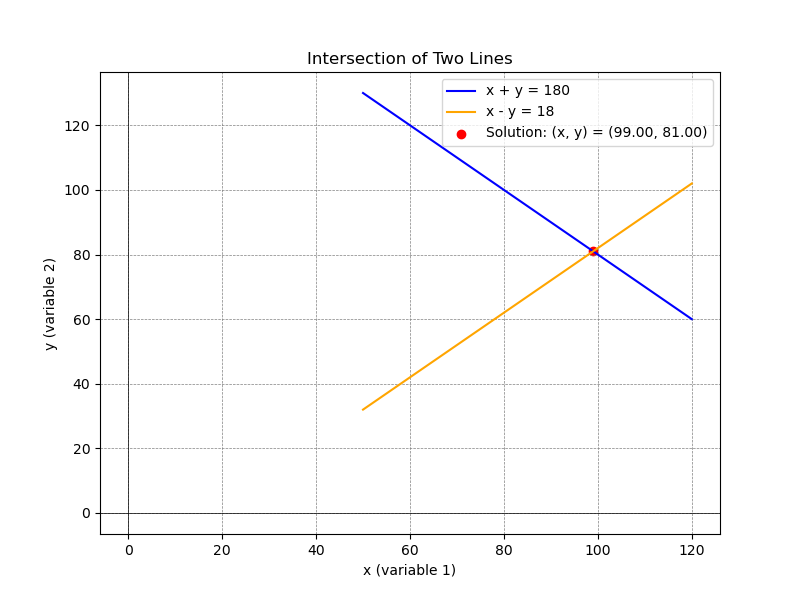
\includegraphics[width=\columnwidth]{figs/figs.png}
\end{figure}

\end{document}
